\documentclass[12pt]{article}
\usepackage[a4paper, margin=1in]{geometry}
\usepackage{amsmath, amssymb}
\usepackage{graphicx}
\usepackage{float}
\usepackage{hyperref}
\usepackage{fancyhdr}
\usepackage{caption}
\usepackage{color}
\usepackage{parskip}
\usepackage{times}
\usepackage{titlesec}

\pagestyle{fancy}
\fancyhf{}
\setlength{\headheight}{14.49998pt}
\lhead{Julia Zimmerman}
\rhead{Institute for Computing in Research}
\cfoot{\thepage}

\titleformat{\section}{\normalfont\large\bfseries}{\thesection}{1em}{}
\titleformat{\subsection}{\normalfont\normalsize\bfseries}{\thesubsection}{1em}{}

\title{\textbf{
Quantifying Sky Signals: Simulating Visibility Correlations in Radio Interferometry
}}
\author{Julia Zimmerman\\Institute for Computing in Research\\July 2025}
\date{}

\begin{document}
\maketitle

\begin{abstract}
This paper explores calculating visibility in radio interferometry, a complex number that encodes amplitude and phase information of radio waves. The paper will discuss the key elements of radio interferometry that help us expand our knowledge of distant astronomical sources. By deriving the total visibility equation for a single baseline at a specific frequency and time, this paper discusses the uses of radio waves in astronomical research and how they can provide more insight into the nature of astronomical objects and their environment. This is done through understanding the radio interferometry simulator, a simple Python simulator built to model visibility using unpolarized light and monochromatic frequencies. Using the Fourier transform on the resulting visibility, the simulation plots the geometric time delay of a set of sources to explore how they move across the sky. 
\end{abstract}

\section{Introduction}

    Human eyes can only detect a small sliver of the electromagnetic spectrum, known as visible light. While visible light serves us well in our day-to-day lives, to understand the cosmos, a more complete spectrum is required. Previously thought to be the only type of light, scientific breakthroughs by notable figures such as Sir William Herschel and Paul Villard \cite{[2]} broadened this band to include wavelengths such as ultraviolet, infrared, and, most notably for this project, radio waves. Radio astronomy allows us to observe details of the universe undetectable under visible light and understand the universe in more detail. 

    Using an array of radio antennas that detect radio waves emitted from distant astronomical sources, radio interferometry addresses one of the main concerns of astronomy: creating precise measurements of the angular positions of astronomical sources \cite{[1]}. An interferometer primarily uses the Fourier transform, also named the fringe visibility function. By calculating the correlation between two or more electrical field measurements, a measurement called visibility is obtained. A radio interferometer then creates detailed angular measurements of radio emissions from outer space \cite{[1]}. Analogous to the two slit experiment, an interferometer observes and measures the interference pattern constructed by multiple apertures \cite{[3]}. With this, astronomical sources are identified with more ease and, more importantly, more accuracy. Additionally, using an array of antennas instead of a single antenna improves the resolution of our observations, heightening accuracy levels \cite{[1]}. 

    This paper presents a simulation of visibility in interferometric applications. Visibility is the 2-dimensional Fourier transform of the brightness of the sky, which is directly linked to the interference pattern measured by an interferometer \cite{[3]}. Visibility is a complex quantity. This is done to store information on both the amplitude and phase of the wave \cite{[3]}. Given this information, multiple types of analysis can be performed, such as geometric time delay interpretations, as done in this paper. This visibility data allows us to understand the source in more detail than what the naked eye can observe using a telescope. 

    This paper will focus on calculating and building a simulation to represent visibility, helping us understand and model how it can be used to do basic radio interferometric analysis. 

    

\section{Methodology}
\subsection{Calculating Visibility}
\label{subsec:visibility}

As mentioned, visibility is a complex number that stores information about the wave's frequency and amplitude. Deriving the visibility starts with the equation for the complex electromagnetic field at a single frequency of a source.

The process uses equation~\ref{eq:1} to derive equation~\ref{eq:4}, which will provide context on how to calculate visibility. 
\begin{equation}
\tilde{E}[\vec{r}, t] = \tilde{E}_0 e^{i(\vec{k} \cdot \vec{r} - \omega t)}
\label{eq:1}
\end{equation}
To begin, $\vec{k}$ represents the wave vector, and is equivalent to $\frac{2\pi}{\lambda}$. $\vec{r}$ is the position vector. $\omega$ can be written as $2\pi\nu$ and represents angular frequency. Finally, $\nu$ represents oscillation frequency. 

Before moving on to equation~\ref{eq:3}, a crucial assumption must be made. The assumption is that the wave is traveling as a plane wave. This drops the dot product apparent in equation~\ref{eq:1}, resulting in the following equation:
\begin{equation}
\tilde{E}_1 = \tilde{E}_0 e^{i(kz - \omega t)}
\end{equation}

From here, one can derive the equation to compute the electromagnetic field. 

First, substitute $\frac{2\pi}{\lambda}$ for $\vec{k}$, and substitute $2\pi\nu$ for $\omega$. Then $2\pi\nu$ gets factored out, and the following equation is derived. 
\begin{equation}
\tilde{E}_1 = \tilde{E}_0 e^{2\pi i \nu \left( \frac{z + d}{c} - t \right)}
\label{eq:3}
\end{equation}
Notice, this equation has an additional $d$ added to $z$. This represents the geometric time delay. Radio waves don't travel to each antenna simultaneously. There are slight delays between each antenna, called the geometric time delay. The $d$ being added to $z$ represents the extra distance, $d$, the wave must travel to reach the second antenna.  

To obtain the visibility for a single source of a single baseline at a specific frequency and time, one must calculate equation~\ref{eq:3} for each of the two antennas, and cross-correlate the two equations together. 

\begin{equation}
\langle \tilde{E}_1 \tilde{E}_2^* \rangle = |\tilde{E}_0|^2 e^{2\pi i \nu \frac{\vec{b} \cdot \hat{s}}{c}}
\label{eq:4}
\end{equation}
Notice, the geometric time delay, while previously denoted as $\frac{d}{c}$, is now represented as $\frac{\vec{b} \cdot \hat{s}}{c}$ instead. This is because these two expressions are equivalent.

For further exploration of how an interferometer works, in Figure~\ref{fig:radio_interferometry_diagram} it's visible that the unit vector $\hat{s}$ points towards the astronomical source. The $\vec{b}$ denotes the baseline between the two antennas, and our time delay, $T_g$, is expressed as $\frac{\vec{b} \cdot \hat{s}}{c}$.
\begin{figure}[H]
    \centering
    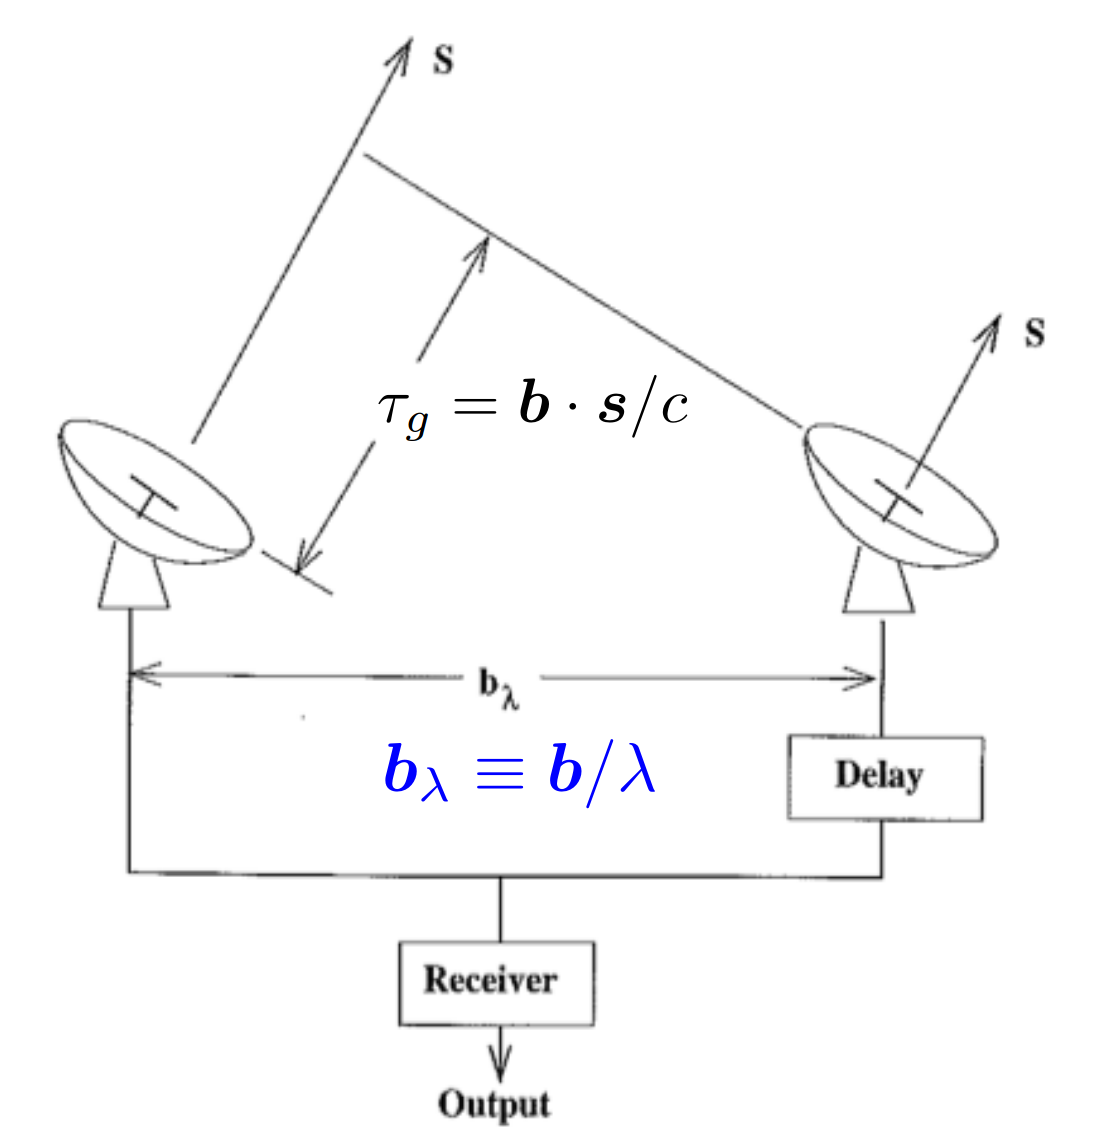
\includegraphics[width=0.5\linewidth]{better_radio_interferometer.png}
    \caption{Diagram of a radio interferometer. The diagram denotes some variables with slight differences in notation.} \cite{[10]}
    \label{fig:radio_interferometry_diagram}
\end{figure}

The cross correlation outputs the visibility for a single source at our single baseline, at a specific frequency and time. To get the total visibility for the entire baseline of every source being observed, one must superpose or add the visibilities of each source together. This is mathematically represented in equation~\ref{eq:5}


\begin{equation}
V_{\text{total}}(\vec{b}, t) =
\sum_{n} |\tilde{E}_{0,n} | ^2
e^{\frac{2 \pi i \nu_n \, \vec{b} \cdot \hat{s}_n(t)}{c}}
\label{eq:5}
\end{equation}

\subsection{Baseline and Unit Vector Calculation}
\label{subsec:vectors}

Mentioned in section~\ref{subsec:visibility}, the baseline and unit vectors are important calculations for the visibility simulation. 

The baseline vector is the vector between the two antennas' positions. The baseline vector can be found by simply subtracting one antenna's position in ENU (East North Up) coordinates from another. It's expressed as $\vec{b} = \vec{r}_2 - \vec{r}_1$.

The unit vector ${\vec{s}}$ represents the direction to the source. This unit vector is calculated through the simulation and is expressed in ENU coordinates. See section~\ref{subsec:python} for how it's computed in the simulation. 

\subsection{Python Modules and Structure}
\label{subsec:python}
The simulation uses the Astropy module to instantiate astronomical sources \cite{[5]}, and antenna array locations \cite{[6]}. The NumPy module was used to create arrays \cite{[7]} to store our data. 

For our analysis, a three-dimensional array stores visibility values, containing baseline, frequency, and time information. 

The antenna locations of the interferometer were created using the EarthLocation class in Astropy by inputting longitude and latitude values. Then, offsets in ENU coordinates were created, centered around the EarthLocation object, to create the positions of the individual antennas. A for loop is used to pair the antennas together, as shown in Figure~\ref{fig:antenna_for_loop}, to calculate all the possible baselines. A crucial component of the for loop is the \texttt{if j != i}. This ensures that antennas don't get paired up with themselves and avoids redundant baselines. Once the antennas are paired, the coordinates of each antenna are subtracted to acquire our baselines. 
\begin{figure}[h]
    \centering
    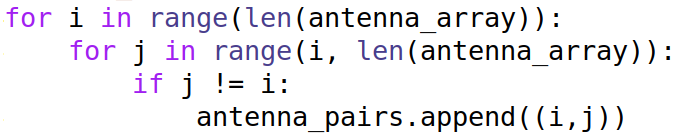
\includegraphics[width=0.5\linewidth]{antenna_for_loop.png}
    \caption{For loop creating antenna pairs. Avoids self-pairings.}
    \label{fig:antenna_for_loop}
\end{figure}

Next, to instantiate a source, the SkyCoord class of Astropy is used. This can be done by inputting the Right Ascension and Declination values of the sources that are being observed. Then, an array is created to store these values. 

The unit vector is calculated through the simulation as well, as mentioned in section~\ref{subsec:vectors}. By inputting the SkyCoord object, the EarthLocation object, and the time of observation in ISO format, the simulation returns a coordinate in ICRS of the unit vector. However, the unit vector is measured in ENU coordinates. To convert an ICRS coordinate to an ENU coordinate, it is first transformed into an Altitude-Azimuth coordinate, using SkyCoord's transform\_to() method. From here, it's converted to a Cartesian coordinate, which results in an x, y, z coordinate. An important factor is that the Cartesian coordinates' output is in NEU form, instead of ENU form. When calling the unit vector calculation method, one must specify the order to rearrange the coordinate value, as shown in figure~\ref{fig:unit_vector}

\begin{figure}[h]
    \centering
    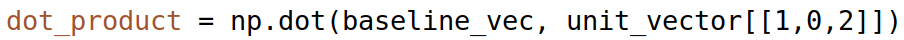
\includegraphics[width=0.75\linewidth]{unit_vector.png}
    \caption{Unit vector calculation showing NEU to ENU coordinate reorganization.}
    \label{fig:unit_vector}
\end{figure}

\subsection{Calculating Visibility Through the Simulation}
Now, visibility can be calculated. The unit and baseline vectors are calculated as mentioned in section~\ref{subsec:vectors} and ~\ref{subsec:python}. Then one dot products the two vectors as mentioned in section~\ref{subsec:visibility}. This dot product is divided by the speed of light, $c$, to represent our geometric time delay. 

Additionally, the simulation requires the amplitude values and frequencies being analyzed.

Using all of these inputs, the simulation computes visibility using the following method.
\begin{figure}[H]
    \centering
    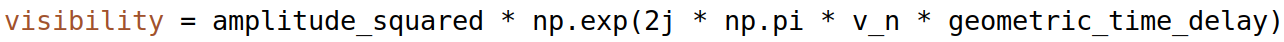
\includegraphics[width=0.8\linewidth]{visibility_equation.png}
    \caption{Code to compute visibility. $v_n$ represents frequency, geometric time delay is the dot product.}
    \label{fig:visibility_code}
\end{figure}

The simulation itself creates an array of the inputted times, frequencies, and the computed baselines to create a three-dimensional array. This array is what stores the outputs of the visibility computations. 

\begin{figure}[h]
    \centering
    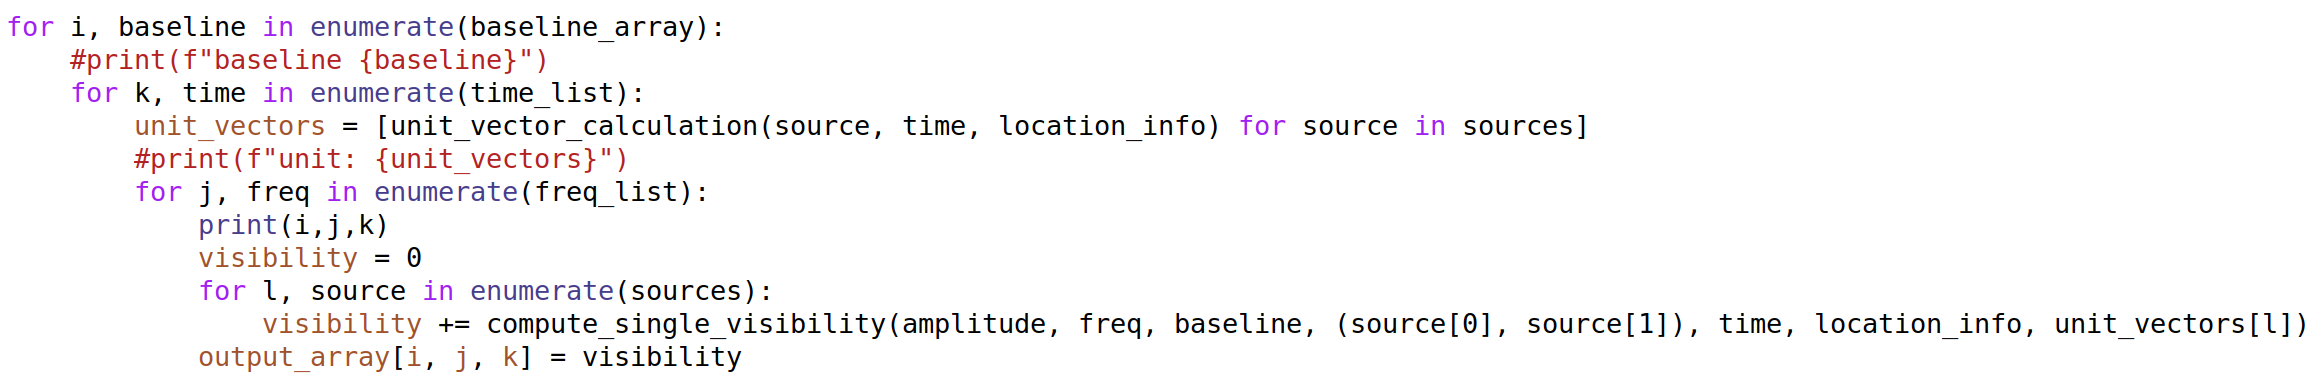
\includegraphics[width=0.8\linewidth]{updated_for_loop.png}
    \caption{For loop, looping through each source, baseline, time, frequency.}
    \label{fig:updated_for_loop}
\end{figure}

In Figure~\ref{fig:updated_for_loop}, one can see that each source is looped through each frequency, time, and baseline. These individual visibilities are then added to the empty visibility variable, which compiles all the calculated visibilities for each source. At the end of the for loop, the total visibility of all of the sources for the single baseline is acquired. These visibilities are then outputted as a 3-dimensional array. 

\section{Results}
\subsection{Geometric Time Delay Analysis}
While many types of analysis can stem from visibility data, one type is geometric time delay analysis. As radio waves reach our baseline composed of two antennas, they hit one of the antennas first. Then, the wave must travel a small extra distance to reach the second antenna. The time it takes to travel this small distance is what is called the geometric time delay. 

First, the simulation is run to create our sources and our baseline. For this analysis, a total of 100,000 frequencies spaced 100 kHz apart were inputted. The data was run at a single time point for an hour; midnight of New Year's Day, 2023, was used. Our antenna array is located at -50.6 longitude and 0 latitude. This data set creates a single baseline, and the antennas are positioned at (0, 0, 0) and (100, 0, 0) offsets of our antenna array location, making our baseline (100, 0, 0). There are 24 sources, 15 degrees apart. Each 15-degree increment represents one hour of the entire 24-hour day (360/24 = 15). These sources range from -180 to 165 degrees in right ascension. Declination values stay 0. This allows the sources to move across the celestial equator horizontally while staying consistent vertically. 

Then, a Fourier transform is used on the resulting frequency visibilities. This converts them from the frequency space to the geometric time delay space. Then, the plot in figure~\ref{fig:time_delay_plot} is generated.
\begin{figure}[H]
    \centering
    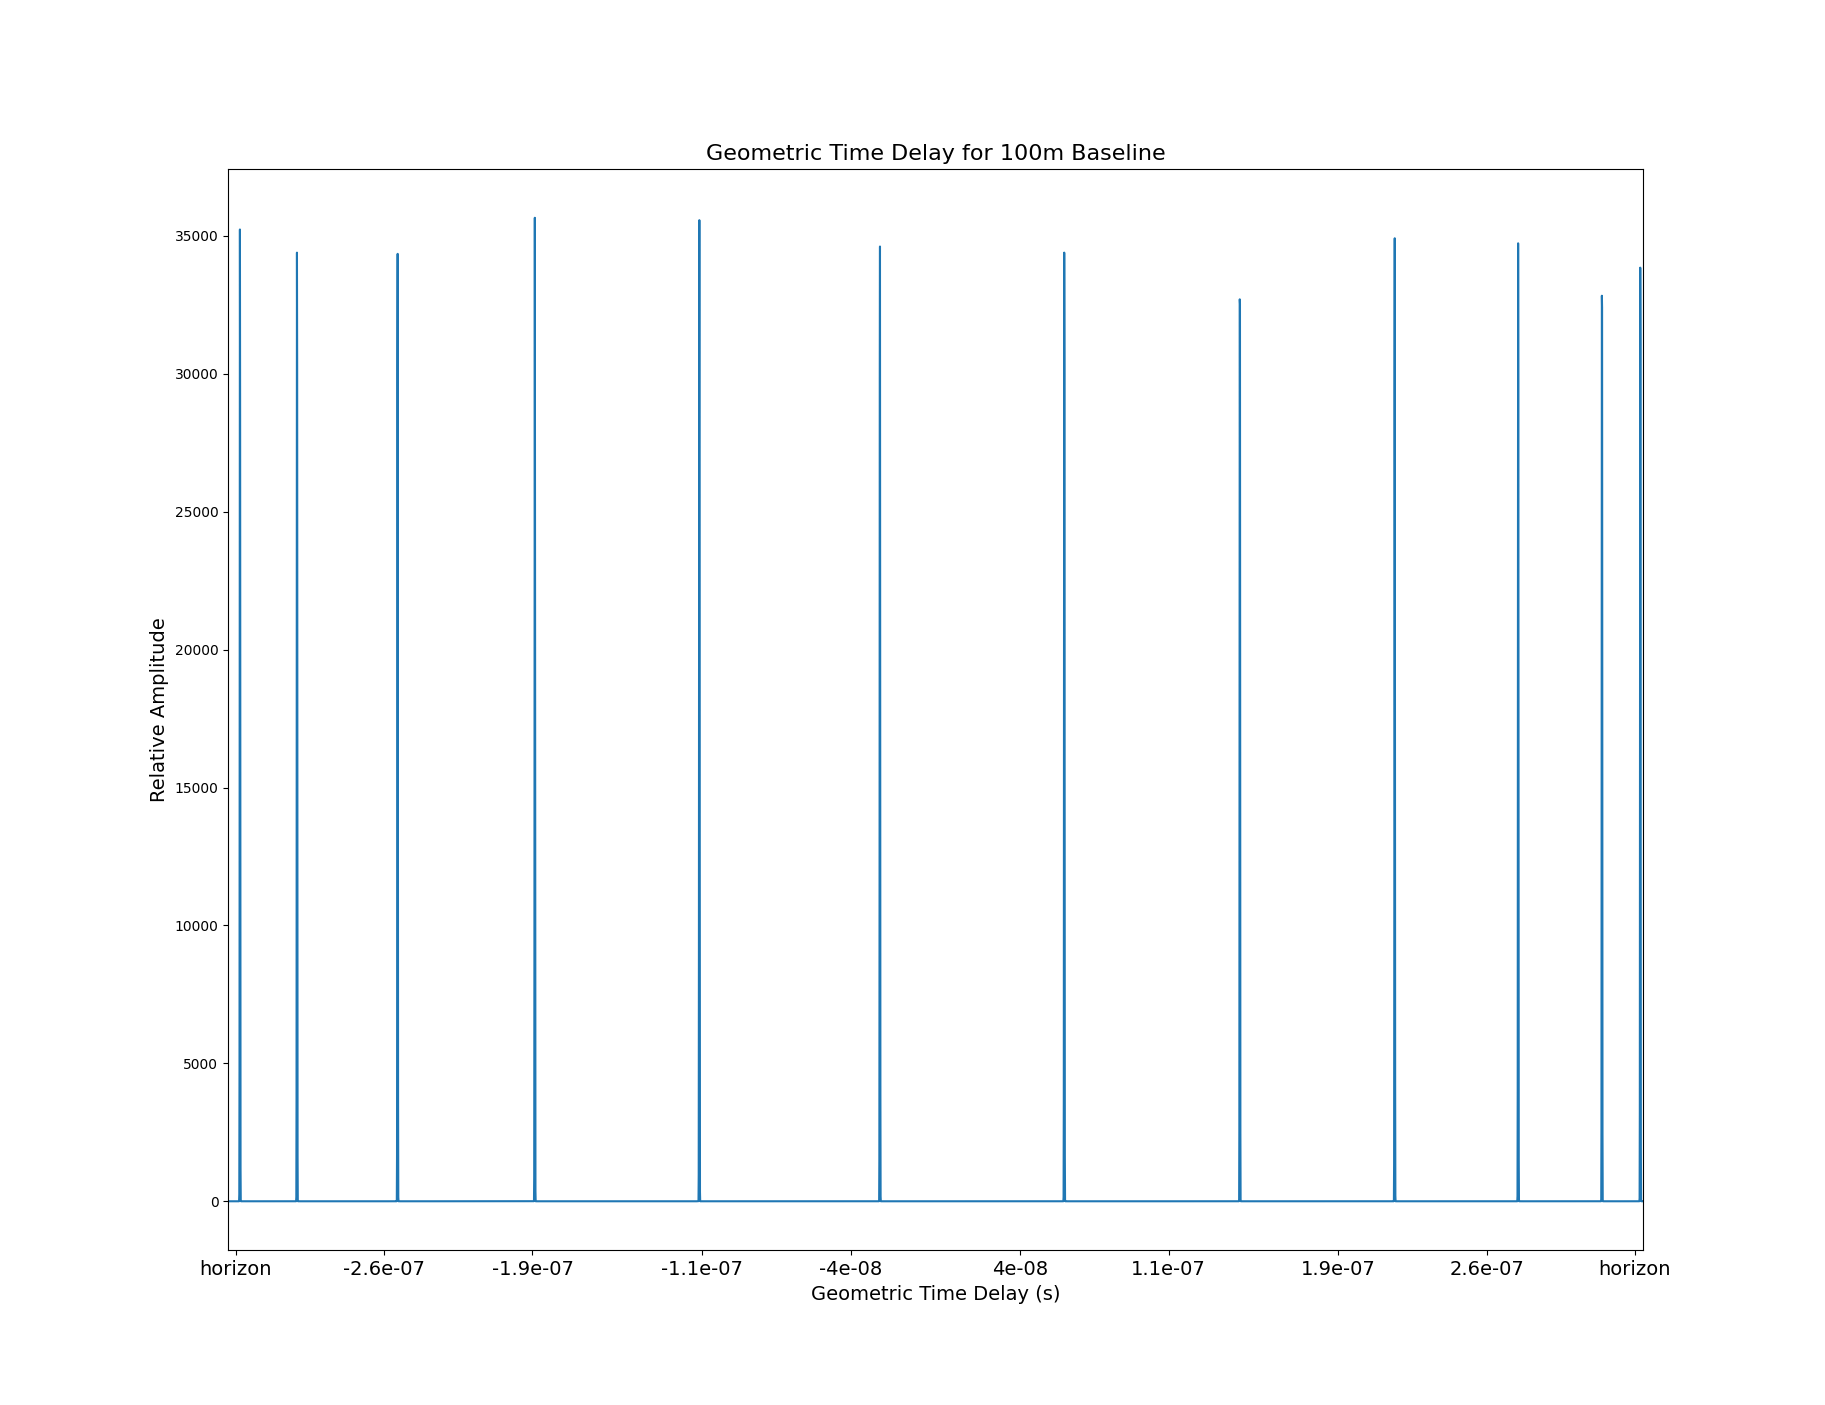
\includegraphics[width=0.75\linewidth]{time_delay_plot.png}
    \caption{Geometric time delay analysis plotted against seconds and relative amplitude.}
    \label{fig:time_delay_plot}
\end{figure}

The x-axis of the plot represents our geometric time delay in seconds. 

The y-axis represents relative amplitude. Each peak corresponds to a delta function, and with higher resolution, these peaks would become taller. Delta functions are infinitely narrow and infinitely tall, but are seen as discrete on our plot as a discrete Fourier transform is being used.

Each spike in figure~\ref{fig:time_delay_plot} represents one of the 24 sources, and its position along the x-axis shows the expected time delay.

When a source is directly overhead, there is no time delay as the radio wave reaches both antennas at the same time. As a source moves closer to the horizon, the geometric time delay increases. This is because one antenna will always be closer to the source when the source isn't directly above the antennas. This requires the wave to travel a small bit of extra distance to reach the secondary antenna, creating a small amount of geometric time delay. A source on the horizon exactly has the maximum possible time delay, which is limited by the baseline length.

Although there are 24 sources spaced 15° apart, only 12 are visible here because the other sources are below the horizon and out of view. 

With all of that being said, one can infer that spikes, or sources, that are closer to the center of the plot have little to no geometric time delay, as these sources are instantiated directly overhead the baseline. The spikes near the outer edges of the plot will have larger geometric time delays, and finally, the two spikes at both ends of the plot have almost the maximum geometric time delay.

This simulation allows us to predict the general geometric time delays of an interferometer, but also allows us to understand how the geometric time delay shifts as sources move across the sky. These results can also double as a way to ensure that our simulation is computing geometric time delay correctly.

\section{Limitations}
\subsection{Simulation vs Reality}
The simulation takes into account unpolarized beams and monochromatic frequencies. The conditions and output that result from the simulation are defined under perfect conditions with no interference. 

In real interferometers, variations in the atmosphere, formation of clouds during observation, circular asymmetries, and pointing errors of antennas are all interferences that can reflect or prevent data collection from the waves \cite{[8]}. While radio waves face interference far less than other areas of the electromagnetic spectrum, such as visible light, it is still affected by interference. This causes the visibility outputs from the simulation to be too idealistic. 

Another limitation of the simulation is that the amplitude is set at 1. This causes all of the sources to have the same brightness if an image was created with the visibility data. This would not be the case for a real interferometer, making this a limitation. 

In a real interferometer, the direction-dependent effects (challenges mentioned previously) decrease the dynamic range of the signals and will make these faraway sources fainter, as they appear in real life \cite{[8]}. 

Finally, this simulation is computationally expensive. The mathematical operations take place one after another; that is, to compute a certain equation, the previous step must be completed. However, most of the calculations are independent of one another. This causes the simulation to run slowly when simulating mass amounts of data, causing it to become computationally expensive. 

\subsection{Improvements to the Simulation}
To make the results of the simulation more similar to the results one would receive in the real world, an important change to the simulation would be to use different amplitudes. This would initially solve the problem of all the sources having the same brightness and allow for analysis of the dynamic range. 

By implementing parallelization, the program can become less computationally expensive. Many of the operations are independent of one another. This allows us to split the computations across multiple cores, allowing calculations to be done simultaneously, speeding up the process.

Finally, a user interface feature, or a method of requesting input from the user to run the simulation, would be a useful addition to make the simulation more approachable. Currently, the simulation can only be run by directly changing the program file. Instead, user input methods could make this simulation a more versatile command-line tool, making it more accessible to a wider range of users. 

\section{Conclusion}
Radio interferometry is a method of observing the sky and understanding more about distant astronomical sources. It provides an array of hidden information that's undetectable when using other parts of the electromagnetic spectrum. The Radio Interferometry simulation takes in information on amplitude, time, frequencies, antenna locations, source positions, and array location to compute visibilities. The outputted visibilities can then be used to understand and plot the geometric time delay and model how sources move across the sky over 24 hours. The outputted data can also be used for a wide range of other analyses, such as reconstructing an image of the sky. 


\section*{Acknowledgements}
I would like to thank my mentor, Mitchell Burdorf, for dedicating his time, knowledge, and efforts to helping me build the simulation, but also for helping me understand basic radio interferometry and its uses. I would also like to thank Dr. Mark Galassi for extending his vast knowledge of research to us, as well as Aaron Grinberg for being at the Portland site and helping all of us interns. I would also like to extend my greatest gratitude to the Institute for providing me with this opportunity to work with my mentor and on this project.


\bibliographystyle{plain}
\bibliography{references}
\end{document}
